\documentclass{article}
\usepackage[utf8]{inputenc}
\usepackage{graphicx}

\title{Reporte 2: Ordenamiento Burbuja\\\textbf{Análisis de Algoritmos}}
\author{ Ramiro Estrada García\\2015190034 }
\date{22 de Octubre del 2020}

\begin{document}
\maketitle
\vspace{5cm}
\section {Características del PC}
\begin{itemize}
	\item CPU: Intel Core i5 9700F a 4.1GHz
	\item RAM: 16GB a 2666MHz
\end{itemize}
\newpage
\maketitle
\section{Mejor caso y peor caso}
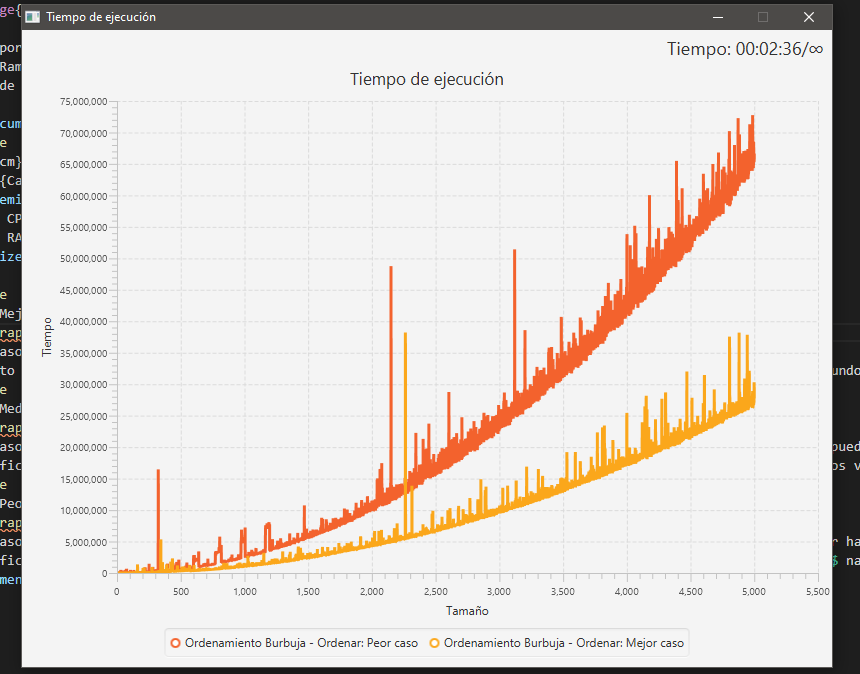
\includegraphics[width=12cm]{mejor-peor.png}
\\ \\
El dominio de las pruebas es $[0, 5000]$. 
En la gráfica se muestra de color rojo el comportamiento del ordenamiento
en peor caso. En este caso, la gráfica tiene un crecimiento cuadratico de
tipo $n^2$ pero la curva es más pronunciada.\\
Por otro lado, de color amarillo, se ve el comportamiento del mejor caso
que sigue siendo de tipo $n^2$ pero su curva es mas plana por lo que se puede
deducir que el algoritmo se encuentra en la misma complejidad pero a uno le toma
más que al otro.
\end{document}